\section{Πλαϊνή Στήλη}
Τώρα στην κατηγορία γενικών στοιχείων στα τα δεξιά του χάρτη βρίσκεται η στήλη με κάποια βασικά δεδομένα όπως φαίνεται στην εικόνα \ref{demo:sidebar}. Καθώς τα δεδομένα είναι πολλά πρέπει ο χρήστης να κυλίσει την σελίδα προς τα κάτω λίγο για να τα δει όλα. 

\begin{figure}[h]
  \centering
  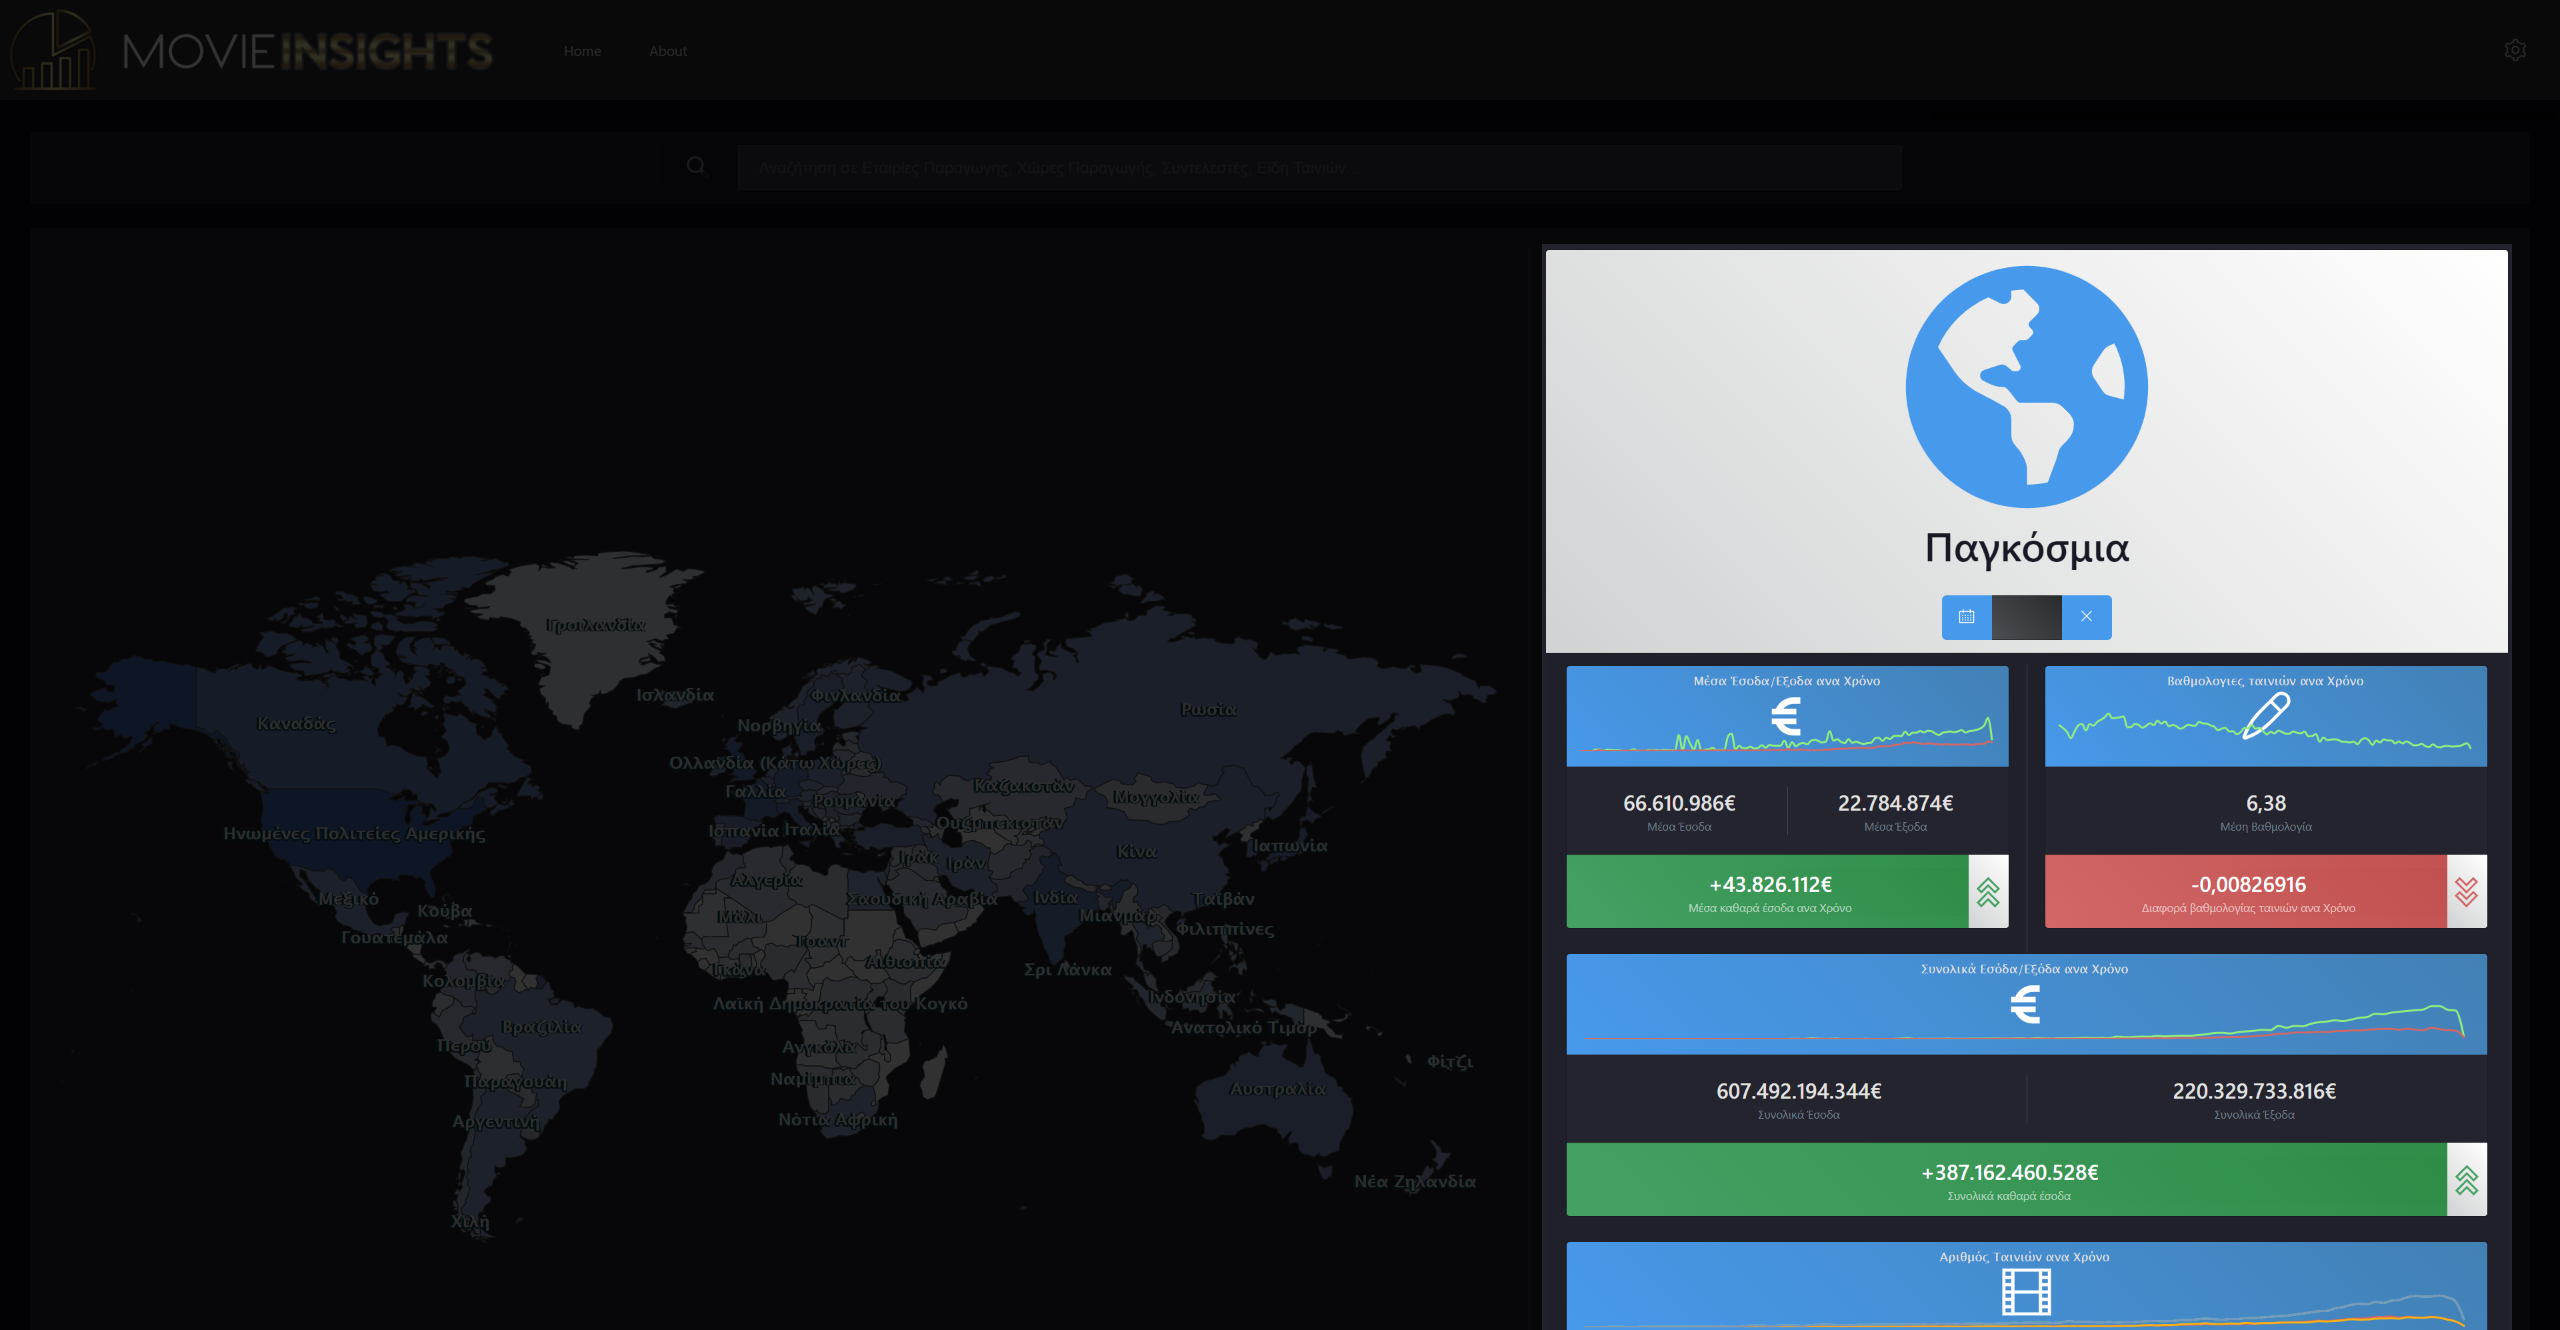
\includegraphics[width=145mm]{Chapters/6 - Manual/Images/main_page_sidebar.png}
  \caption{Πλαϊνή στήλη}
  \label{demo:sidebar}
\end{figure}

Στο πάνω το άσπρο μέρος της πλαϊνής στήλης, όπως φαίνεται στην εικόνα \ref{demo:sidebar_top}, βρίσκονται τα στοιχεία για το ποία κατηγορία βλέπουμε αυτήν την στιγμή που στην παρούσα κατάσταση είμαστε στην κατηγορία γενικών στοιχείων.
Περιέχει μια εικόνα που περιγράφει την κατηγορία που βρισκόμαστε στην προκειμένη περίπτωση καθώς είμαστε στα γενικά στοιχεία έχει επιλεγεί να εμφανιστεί μια υδρόγειος, περιέχει το όνομα της κατηγορίας που στην προκειμένη περίπτωση στην κατηγορία γενικών στοιχείων το όνομα είναι "Παγκόσμια" και περιέχει ένα πεδίο που επιτρέπει στον χρήστη να επιλέξει, είτε πατώντας στο εικονίδιο του ημερολογίου, είτε πατώντας στο πεδίο εισαγωγής, ένα έτος για να δει τα στοιχεία της κατηγορίας ανά έτος. Στα δεξιά του πεδίου εισαγωγής υπάρχει ένα εικονίδιο με το σύμβολο "X" που επιτρέπει τον χρήστη να καθαρίσει την επιλογή έτους για να δει ξανά τα συνολικά δεδομένα.

\begin{figure}[h]
  \centering
  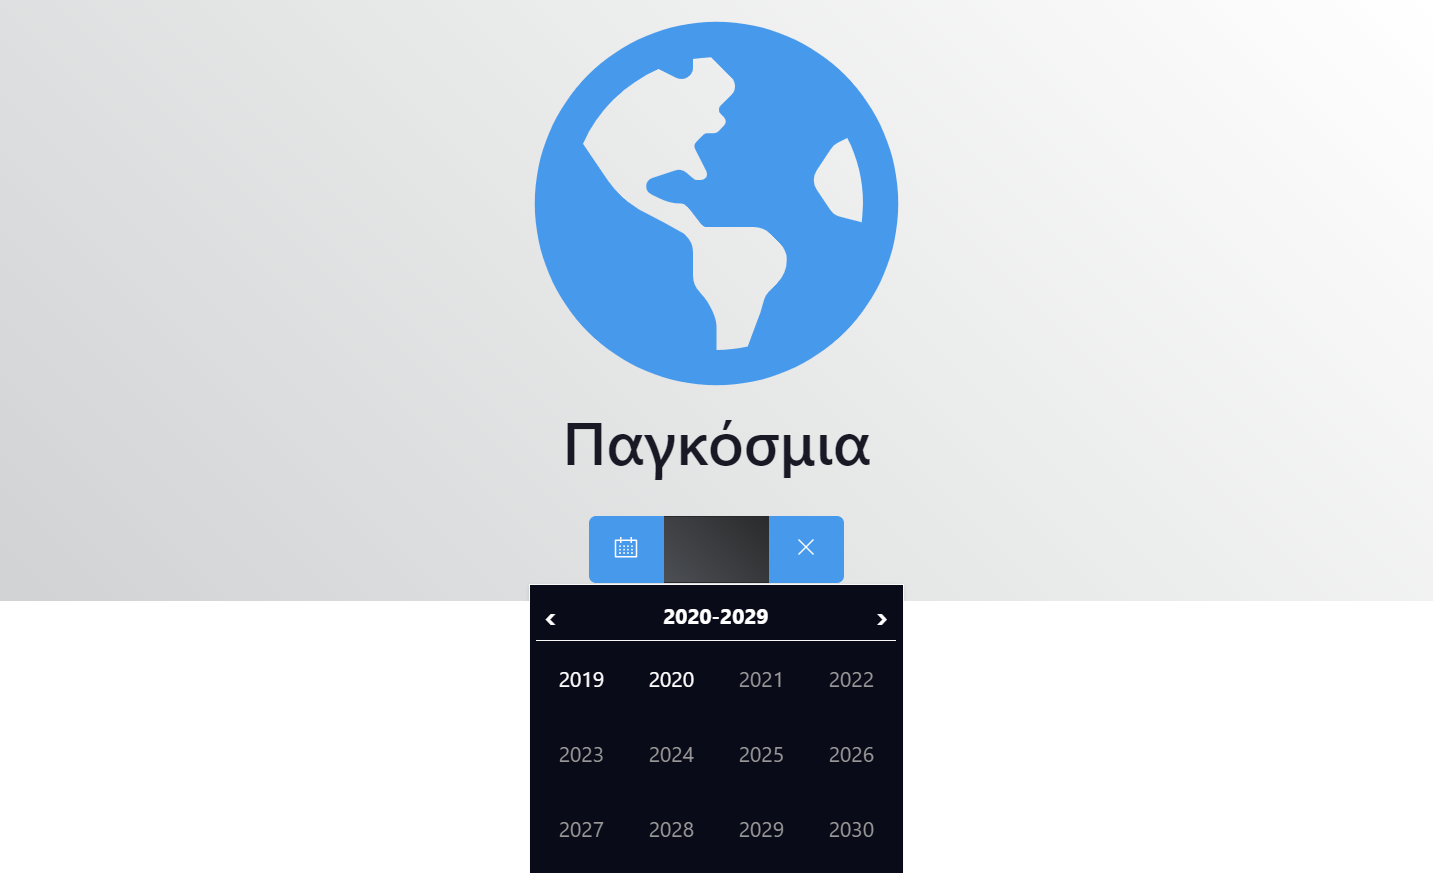
\includegraphics[width=75mm]{Chapters/6 - Manual/Images/main_page_sidebar_top.png}
  \caption{Πάνω μέρος πλαϊνής στήλης}
  \label{demo:sidebar_top}
\end{figure}

Στο πάνω μέρος της πλαϊνής στήλης όταν η κατηγορία είναι οποιαδήποτε άλλη πέρα των γενικών στοιχειών στο πάνω δεξιό μέρος εμφανίζεται ένα κουμπί με το σύμβολο "X", όπως φαίνεται στην εικόνα \ref{demo:sidebar_top_x}, το οποίο όταν πατηθεί επαναφέρει τον χρήστη στην κατηγορία γενικών στοιχείων. 

\begin{figure}[h]
  \centering
  
\includegraphics[width=110mm]{Chapters/6 - Manual/Images/main_page_sidebar_top_x.png}
  \caption{Κουμπί "Χ" στο πάνω μέρος πλαϊνής στήλης}
  \label{demo:sidebar_top_x}
\end{figure}

Το πάνω μέρος της πλαϊνής στήλης παραμένει το ίδιο για όλες τις κατηγορίες εκτός της κατηγορίας "ανά άτομο". Όταν η κατηγορία αναφέρεται σε ένα άτομο εμφανίζεται ένα ακόμα στοιχείο πάνω από το στοιχείο επιλογής έτους. Η εφαρμογή συλλέγει δεδομένα για ένα άτομο σε κατηγορίες. Συλλέγει δεδομένα για το άτομο σαν ηθοποιό, σαν παραγωγό, σαν σκηνοθέτη και σαν συγγραφέα. Για αυτό το λόγο σε εκείνο το σημείο υπάρχουν 4 κουμπιά που σου επιτρέπουν να επιλέξεις να δεις στοιχεία για ένα άτομο σε διαφορετικό ρόλο όπως φαίνεται στην εικόνα \ref{demo:sidebar_top_person}. Από προεπιλογή επιλέγεται ο ρόλος με τον οποίο εμφανίζεται πιο συχνά το άτομο αυτό. Δεν γίνεται να μην επιλεγεί κανένας ρόλος καθώς τα δεδομένα είναι διαφορετικά και βγαίνουν διαφορετικά συμπεράσματα για την πορεία του συγκεκριμένου ατόμου σε κάθε ρόλο. Όταν επιλεγεί ένας ρόλος το κουμπί που κρατάει αυτόν τον ρόλο θα γίνει μπλε. Όταν ένας ρόλος δεν είναι επιλεγμένος είναι σκούρο γκρι. Βέβαια ένα άτομο μπορεί να μην έχει γίνει για παράδειγμα ποτέ συγγραφέας ταινίας η σκηνοθέτης. Όταν λοιπόν δεν υπάρχουν δεδομένα για το συγκεκριμένο άτομο για έναν συγκεκριμένο ρόλο, το κουμπί που κατέχει αυτόν τον ρόλο θα απενεργοποιηθεί και θα χρωματιστεί με χρώμα ανοιχτό γκρι. Στην εικόνα βλέπουμε την ηθοποιό Margot Robbie, με προεπιλεγμένο ρόλο "ACTOR" για ηθοποιό και με έναν διαθέσιμο ακόμα ρόλο "PRODUCER", παραγωγό που σημαίνει ότι η εφαρμογή έχει στοιχεία για την Margot Robbie σαν ηθοποιό και σαν παραγωγό ταινιών αλλά δεν έχει δεδομένα σαν συγγραφέα η σκηνοθέτη. 

\begin{figure}[h]
  \centering
  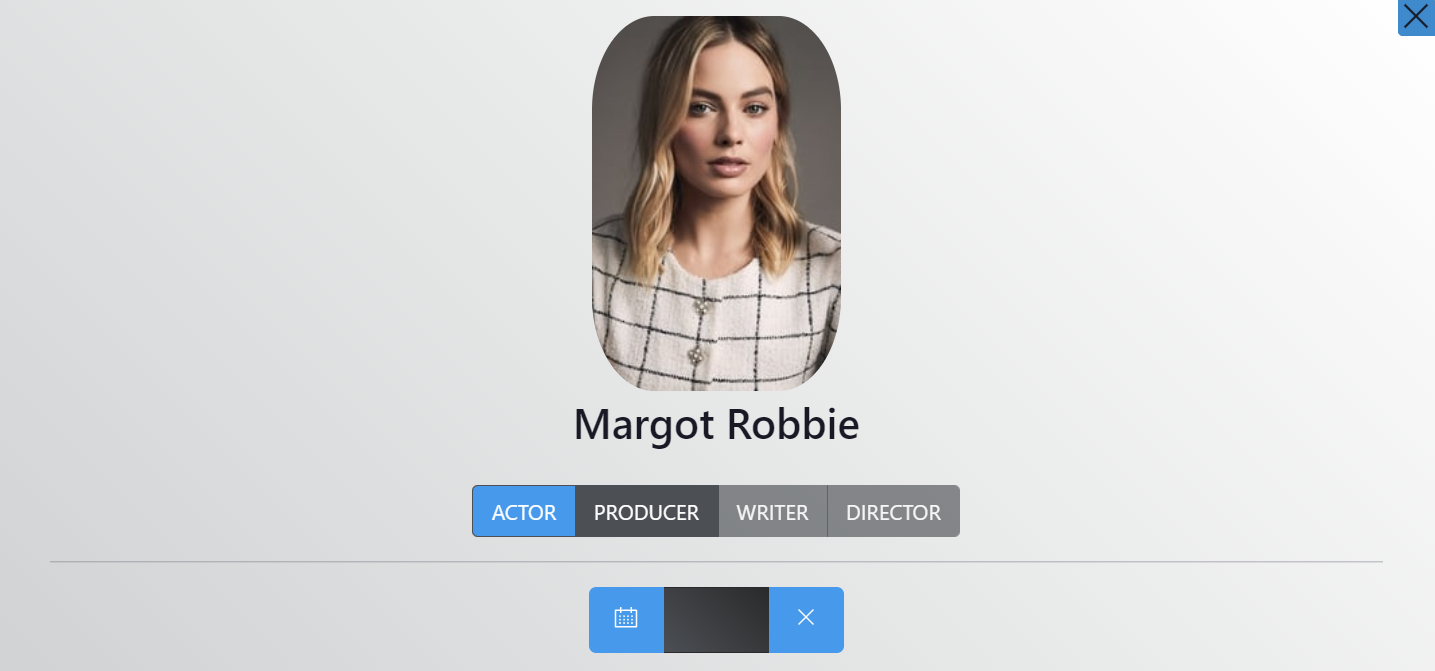
\includegraphics[width=110mm]{Chapters/6 - Manual/Images/main_page_sidebar_top_person.png}
  \caption{Επιλογή Ρόλου στο πάνω μέρος πλαϊνής στήλης}
  \label{demo:sidebar_top_person}
\end{figure}

Στο κάτω μέρος της πλαϊνής στήλης βρίσκονται 4 κάρτες δεδομένων όπως φαίνεται στην εικόνα \ref{demo:sidebar_bottom}.

\begin{figure}[h]
  \centering
  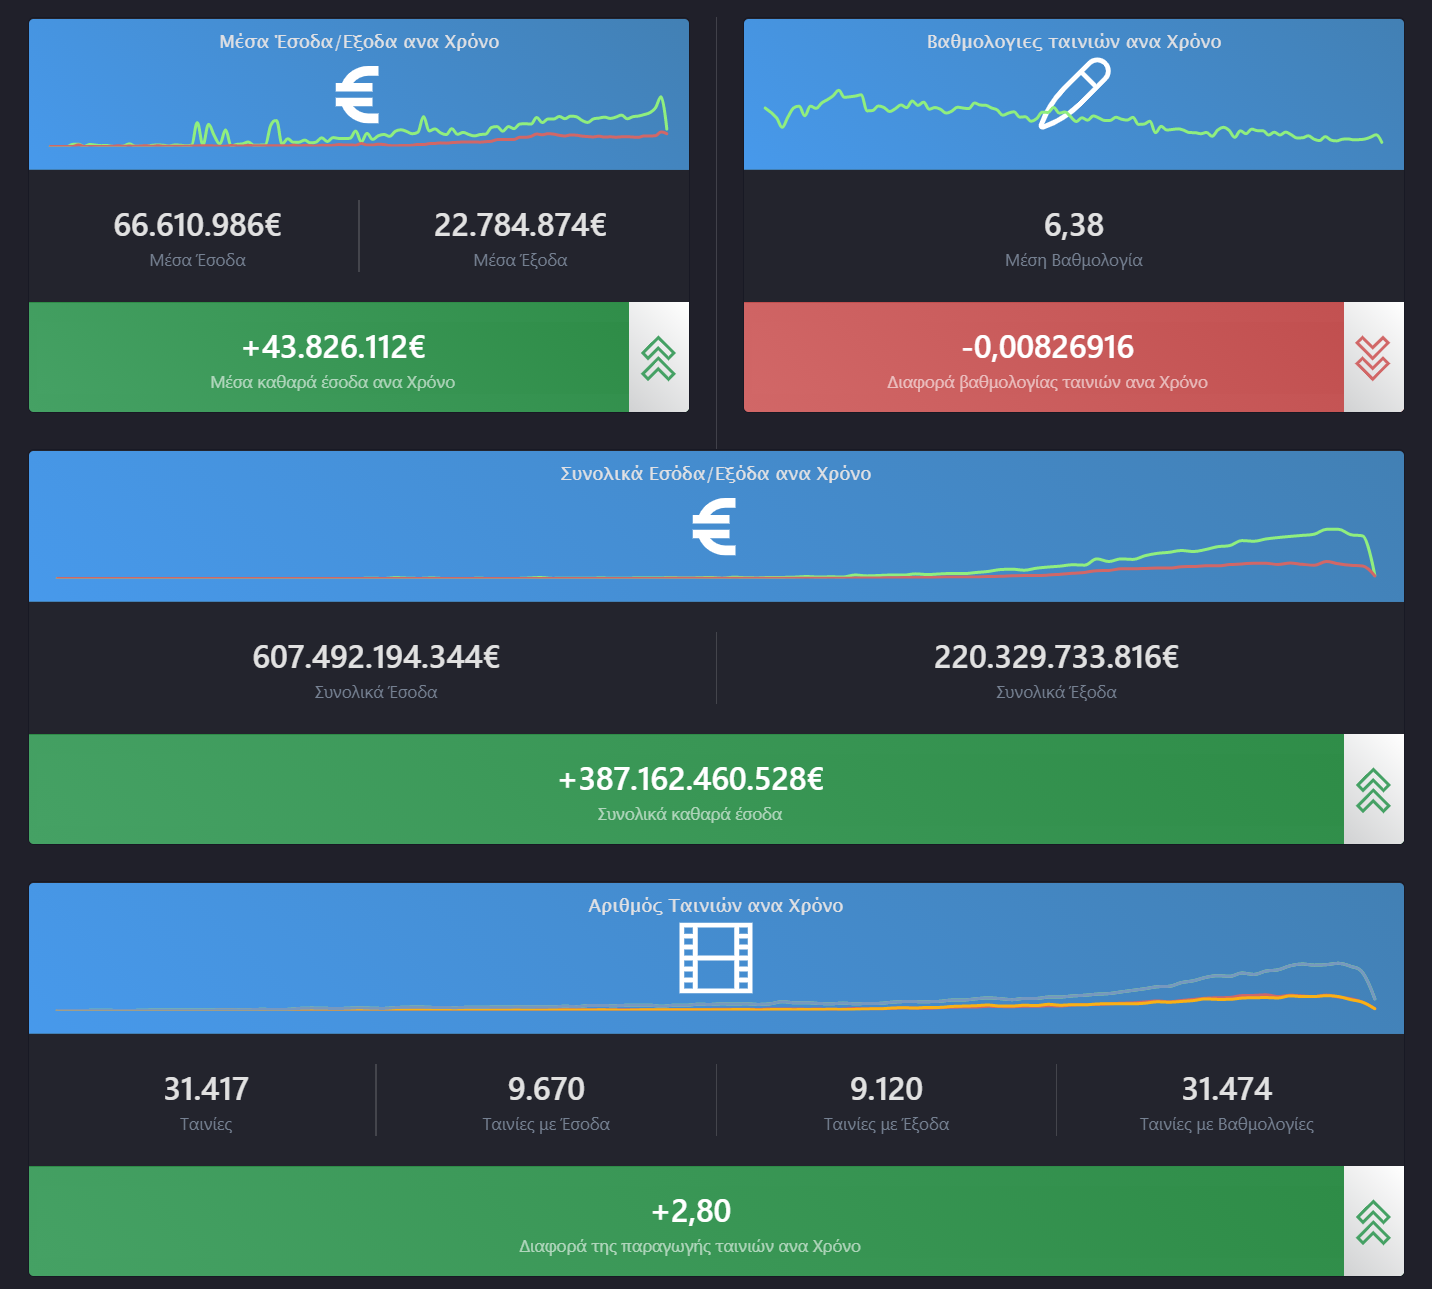
\includegraphics[width=75mm]{Chapters/6 - Manual/Images/main_page_sidebar_bottom.png}
  \caption{Πάνω μέρος πλαϊνής στήλης}
  \label{demo:sidebar_bottom}
\end{figure}

Η κάθε κάρτα περιέχει 3 κομμάτια και 4 καταστάσεις όπως φαίνεται στο σχήμα \ref{demo:sidebar_card}. Το πρώτο κομμάτι πάνω πάνω είναι ένα γράφημα το οποίο περιέχει ένα η περισσότερα ποσοτικά δεδομένα ανα χρόνο, τον τίτλο του γραφήματος για να γνωρίζει ο χρήστης τι κοιτάει καθώς και ένα περιγραφικό εικονίδιο για να γνωρίζει ο χρήστης τι είναι τα ποσοτικά δεδομένα που κοιτάει. Απο κάτω βρίσκεται το δεύτερο κομμάτι το οποίο περιέχει ενα η περισσότερα ποσοτικά δεδομένα που συνήθως είναι είτε τα μέγιστα, είτε τα ελάχιστα, είτε οι μέσοι όροι των δεδομένων των γραφημάτων. Το τρίτο και τελευταίο κομμάτι είναι ακριβώς απο κάτω και εμφανίζει συνήθως μια διαφορά τιμών ή έναν υπολογισμό δεδομένων με βάση τα προηγούμενα. 

\begin{figure}[h]
    \centering
    \begin{subfigure}[b]{0.475\textwidth}
        \centering
        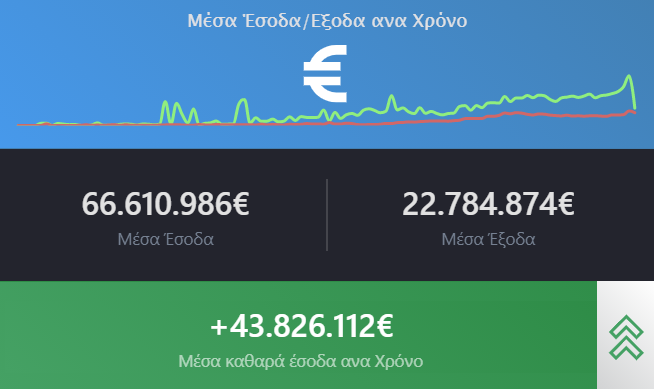
\includegraphics[width=\textwidth]{Chapters/6 - Manual/Images/main_page_sidebar_card_state1.png}
        \caption{Πρώτη κατάσταση}
        \label{demo:sidebar_card:state1}
    \end{subfigure}
    \hfill
    \begin{subfigure}[b]{0.475\textwidth}  
        \centering 
        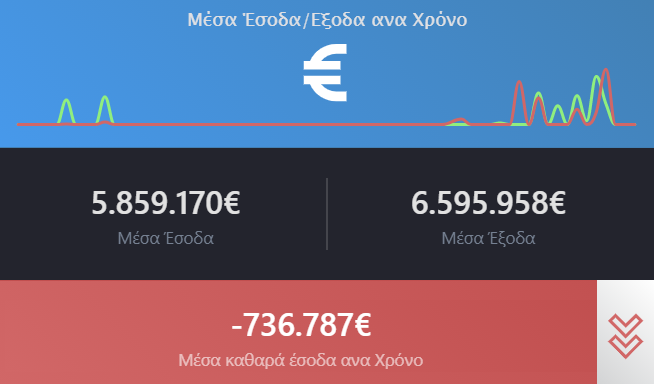
\includegraphics[width=\textwidth]{Chapters/6 - Manual/Images/main_page_sidebar_card_state2.png}
        \caption{Δεύτερη κατάσταση}
        \label{demo:sidebar_card:state2}
    \end{subfigure}
    \vskip\baselineskip
    \begin{subfigure}[b]{0.475\textwidth}   
        \centering 
        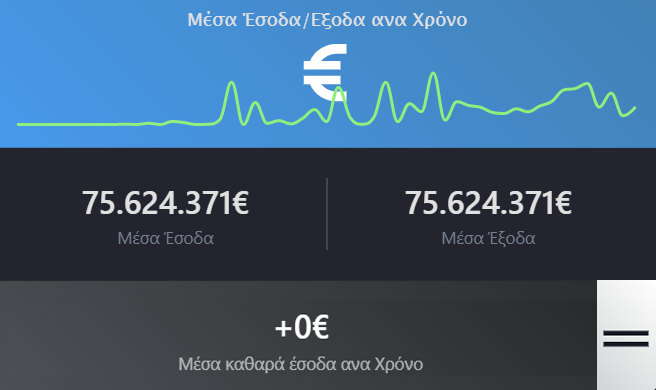
\includegraphics[width=\textwidth]{Chapters/6 - Manual/Images/main_page_sidebar_card_state3.png}
        \caption{Τρίτη κατάσταση}
        \label{demo:sidebar_card:state3}
    \end{subfigure}
    \hfill
    \begin{subfigure}[b]{0.475\textwidth}   
        \centering 
        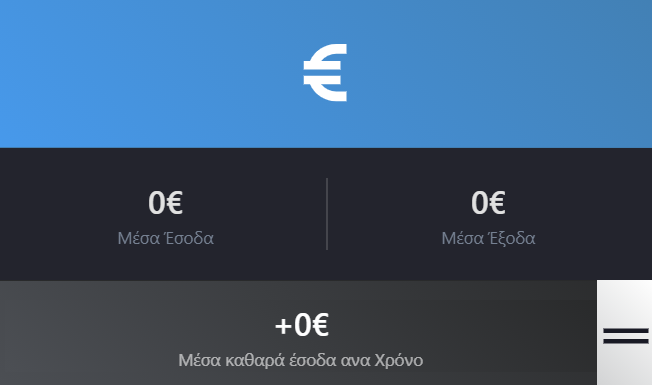
\includegraphics[width=\textwidth]{Chapters/6 - Manual/Images/main_page_sidebar_card_state4.png}
        \caption{Τέταρτη κατάσταση}
        \label{demo:sidebar_card:state4}
    \end{subfigure}
    \caption{Οι κάρτες της πλαϊνής στήλης και οι καταστάσεις τους}
    \label{demo:sidebar_card}
\end{figure}

Όπως προαναφέρθηκε μια κάρτα μπορεί να έχει 4 διαφορετικές καταστάσεις. Όταν η κατηγορία που βλέπει ο χρήστης έχει φιλτραριστεί ανά έτος τότε όλα τα γραφήματα όλων των καρτών, στο πρώτο κομμάτι, που αναφέρουν στοιχεία ανά χρόνο θα σβηστούν και ανάλογα με το τι δείχνει η κάρτα, τα άλλα 2 κομμάτια θα έχουν δεδομένα είτε θα μηδενιστούν όπως φαίνεται στην Κατάσταση 4 στο σχήμα \ref{demo:sidebar_card:state4}. Όταν δεν είναι φιλτραρισμένη η κατηγορία ανά έτος, αν το δεδομένο στο τρίτο κομμάτι της κάρτας είναι θετικό θα έχει χρώμα background πράσινο και στα δεξιά θα έχει ενα εικονίδιο με 2 βελάκια να δείχνουν προς τα πάνω όπως φαίνεται στο σχήμα της πρώτης κατάστασης \ref{demo:sidebar_card:state1}, αν είναι αρνητικό το χρώμα background θα είναι κόκκινο και στα δεξιά θα έχει ένα εικονίδιο με 2 βελάκια να δείχνουν προς τα κάτω όπως φαίνεται στο σχήμα της δεύτερης κατάστασης \ref{demo:sidebar_card:state2}, και αν είναι μηδέν τότε το χρώμα background θα είναι γκρι και το εικονίδιο στα δεξιά θα είναι 2 οριζόντιες γραμμές σαν το σύμβολο "ίσον" των μαθηματικών, όπως φαίνεται στο σχήμα της τρίτης κατάστασης \ref{demo:sidebar_card:state3}.

Η πρώτη κάρτα στην πλαϊνή στήλη εμφανίζει στο γράφημα τα μέσα έσοδα και τα έξοδα όλων των ταινιών στην συγκεκριμένη κατηγορία, και πιο συγκεκριμένα καθώς η κατηγορία η αρχική είναι τα συνολικά δεδομένα, εμφανίζει τα μέσα έσοδα / έξοδα όλων των ταινιών της βάσης δεδομένων. Αν ο χρήστης πάει τον κένσορα πάνω από το γράφημα εμφανίζεται ένα μικρό παράθυρο πάνω από τον κένσορα που αναγράφει το έτος και τα μέσα έσοδα έξοδα του έτους για την τοποθεσία που βρίσκεται ο κένσορας όπως φαίνεται στο σχήμα \ref{demo:sidebar_card:hover}. Απο κάτω αναφέρονται συνολικά κατά μέσο όρο τα μέσα έσοδα και έξοδα των ταινιών και στο τρίτο κομμάτι εμφανίζεται το μέσο καθαρό κέρδος των ταινιών συνολικά.

\begin{figure}[H]
  \centering
  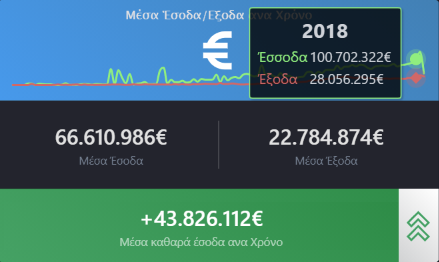
\includegraphics[width=75mm]{Chapters/6 - Manual/Images/main_page_sidebar_card_hover.png}
  \caption{Η Κάρτα με το παράθυρο απο πάνω}
  \label{demo:sidebar_card:hover}
\end{figure}

Στην δεύτερη κάρτα στο γράφημα εμφανίζονται οι μέσες βαθμολογίες των ταινιών ανά έτος. Στο δεύτερο κομμάτι εμφανίζεται συνολικά η μέση αξιολόγηση όλων των ταινιών της κατηγορίας και στο τρίτο κομμάτι εμφανίζεται η τάση των βαθμολογιών ανά χρόνο. Αυτό σημαίνει αν οι ταινίες μέσα στο πέρασμα των χρώνων έγιναν καλύτερες η χειρότερες. Αυτά τα δεδομένα φαίνονται στην εικόνα \ref{demo:sidebar_card:vote}.

\begin{figure}[H]
  \centering
  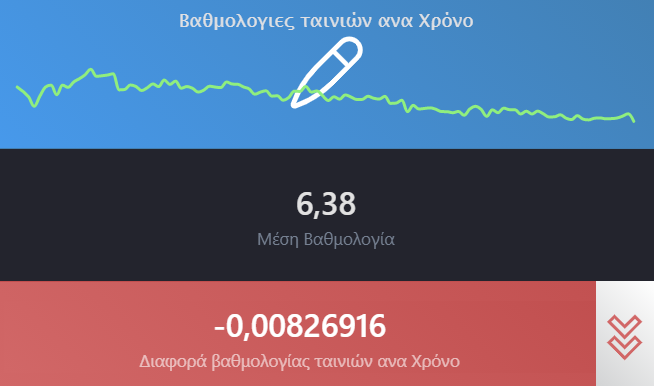
\includegraphics[width=75mm]{Chapters/6 - Manual/Images/main_page_sidebar_vote_card.png}
  \caption{Η Κάρτα βαθμολογιών}
  \label{demo:sidebar_card:vote}
\end{figure}

Η τρίτη κάρτα είναι ακριβώς το ίδιο με την πρώτη κάρτα με την διαφορά ότι αντί για τους μέσους εμφανίζει τα συνολικά δεδομένα, και η τέταρτη κάρτα αναγράφει κάποια στοιχεία για το νούμερο των ταινιών που υπάρχουν στην βάση δεδομένων και πόσες από αυτές παρέχουν δεδομένα εσόδων, εξόδων και βαθμολογιών.